\section{Vorlesung 12: Deep Learning}
\label{sec:vl12}

\subsection{Neural Networks}
\label{subsec:vl12}

\begin{figure}[th]
\centering
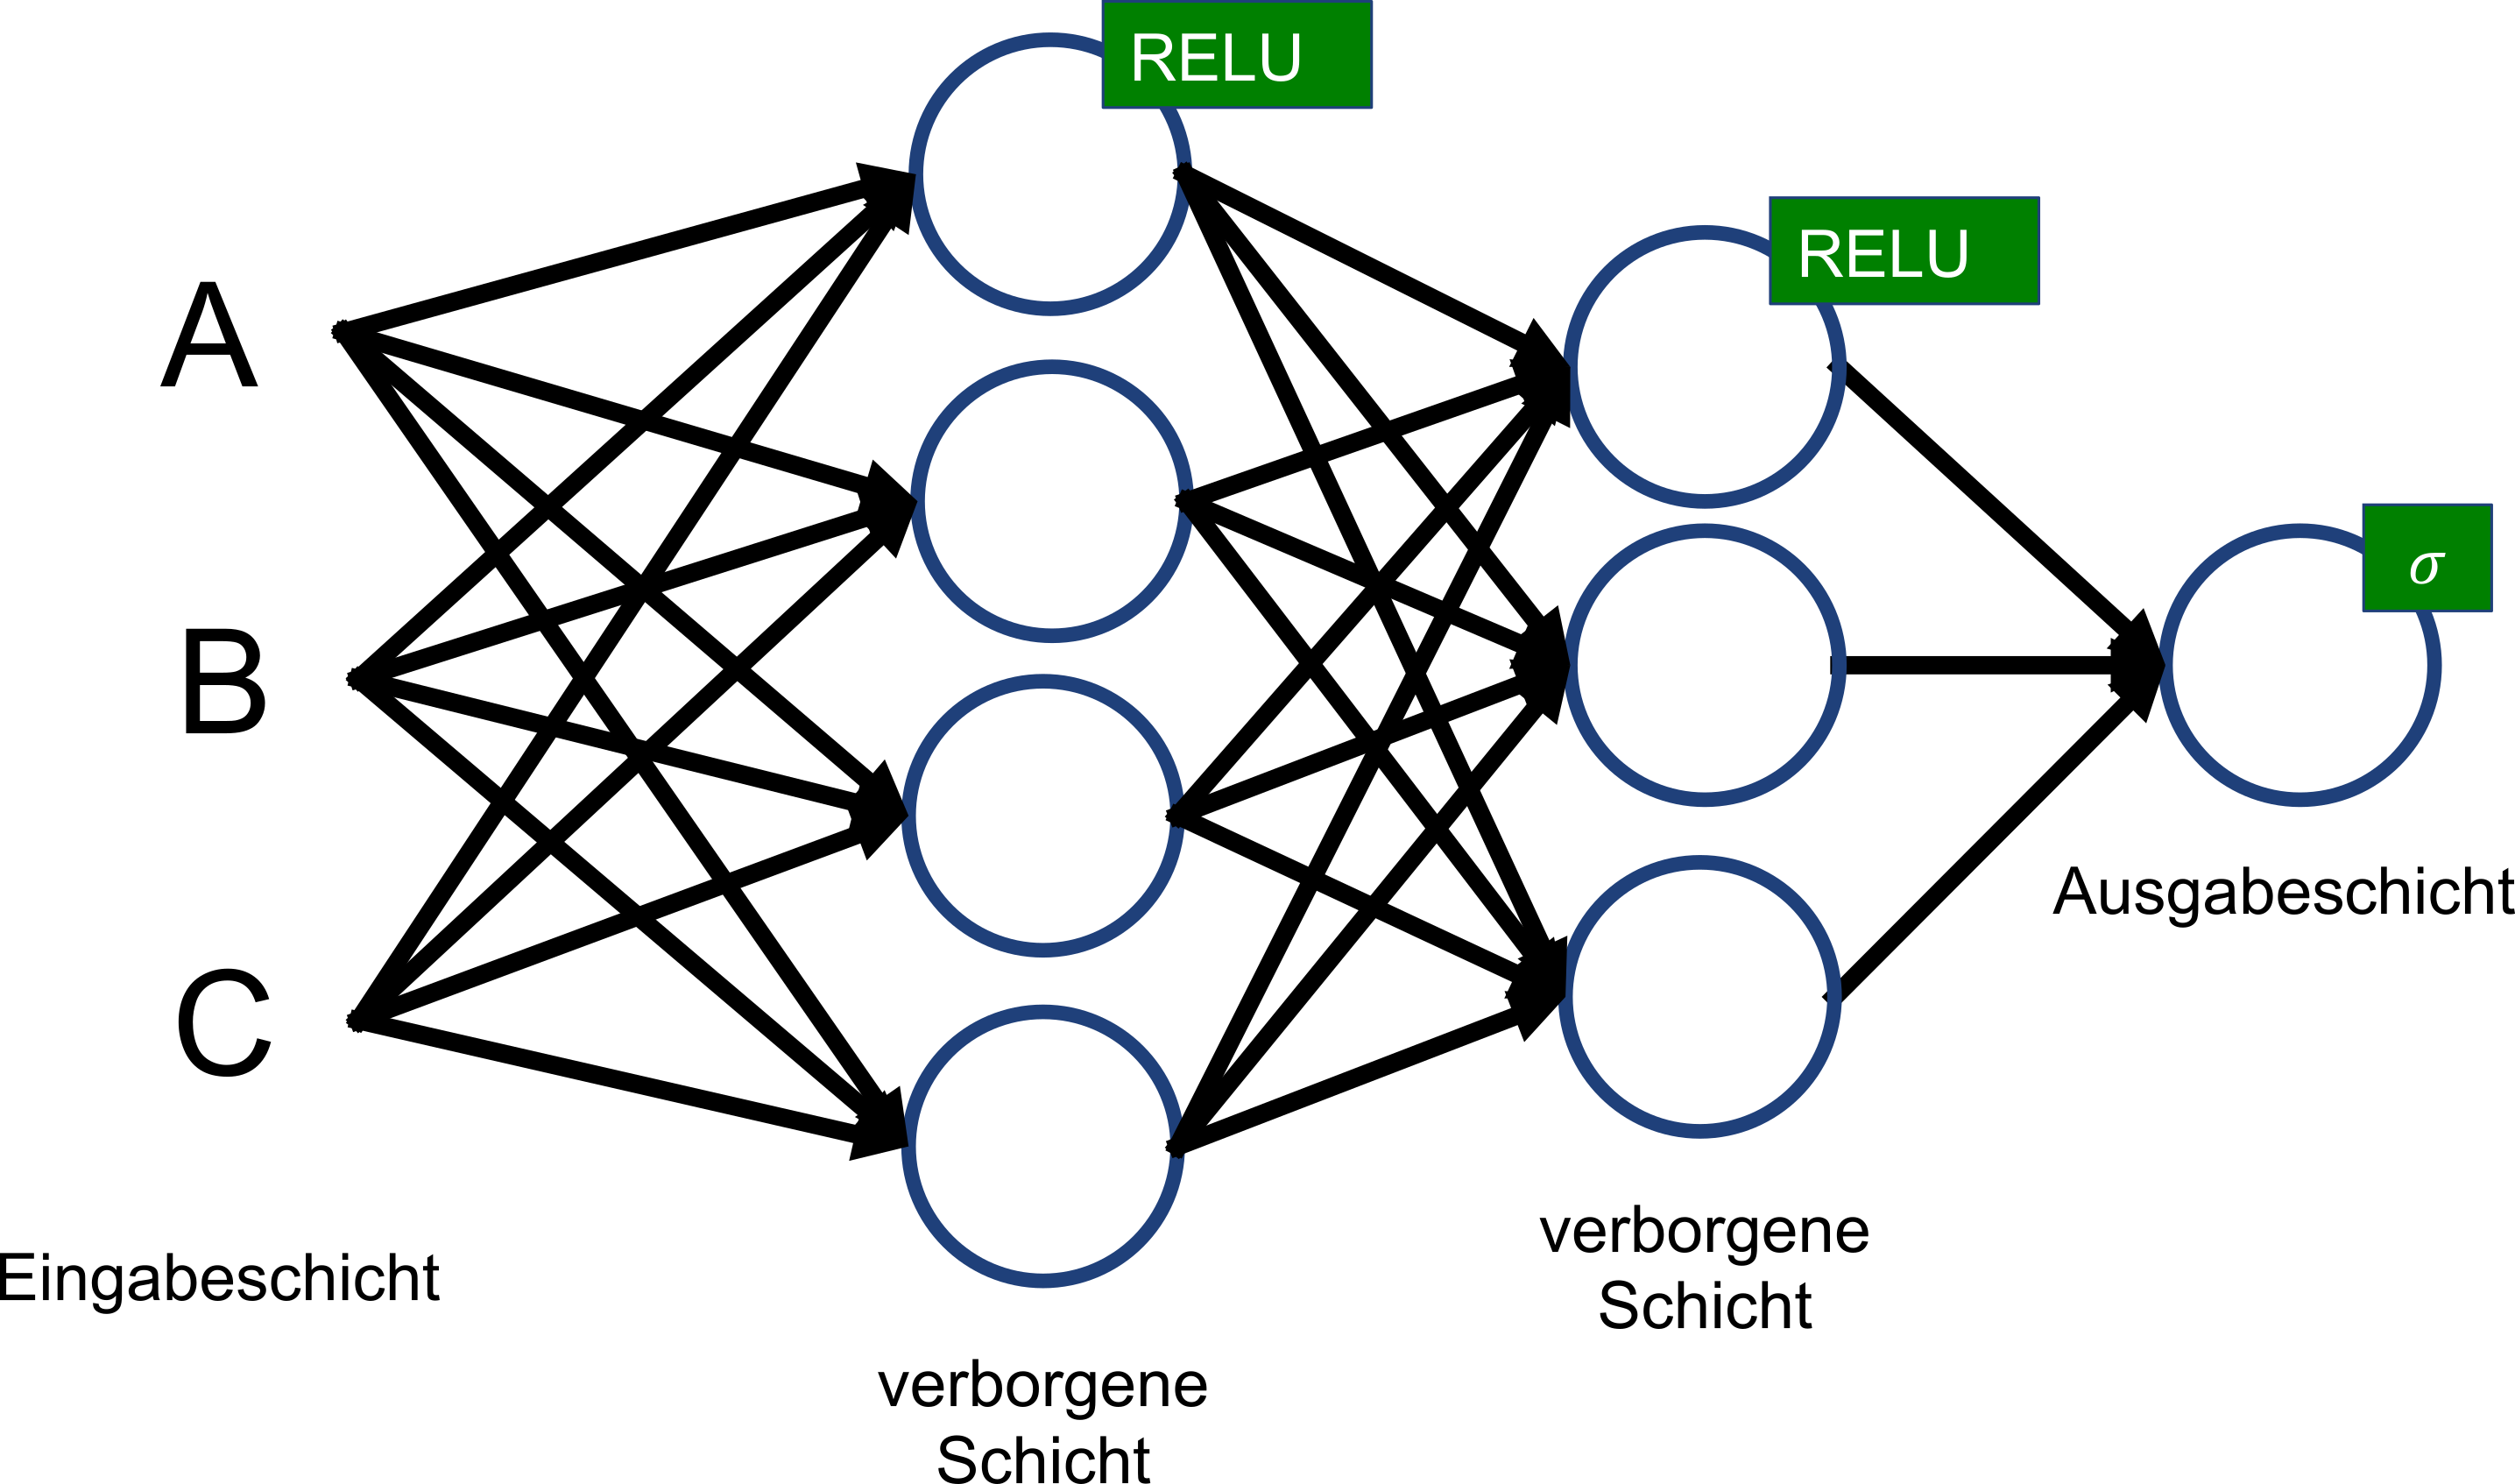
\includegraphics[width=.50\textwidth]{Lectures/VL12_NN_sketch.png}
\caption{Die allgemeine Architektur eines neuronalen Netzes.}
\label{fig:vl12fig1}
\end{figure}

Ein k\"unstliches neuronales Netz ist ein Deep Learning-Computermodell, das biologisches Lernen nachempfindet. %Das Design von Deep Learning-Modellen ist durch das biologische Gehirn inspiriert (menschlich oder tierisch). Dabei sind sie aber nicht so designt, realistische Modelle der biologischen Funktion zu sein.
Deep Learning wird durch zwei Punkte motiviert:

\begin{itemize}
    \setlength\itemsep{0em}
        \item Intelligenz zu erschaffen, indem die Berechnungsprinzipien des Gehirns umgekehrt entwickelt und seine Funktionalität dupliziert wird.
        \item Das Verst\"andnis des Gehirns und die Prinzipien, auf denen Intelligenz basiert, zu erforschen.
\end{itemize}

 Das bis heute anhaltende Interesse f\"ur neuronale Netze begann 2006, als Geoffrey Hinton eine effiziente Strategie zum Trainieren von neuronalen Netzen fand.\\
 Obige Informationen entnommen aus: \textit{Ian Goodfellow, Yoshua Bengio, Aaron Courville (2016). ``Deep Learning'', MIT Press, \url{http://www.deeplearningbook.org}.}\\[0.3cm]
 Ein neuronales Netz ist in \cref{fig:vl12fig1} visualisiert. Es besteht aus einer Eingabeschicht, Ebenen von verborgenen Schichten und einer Ausgabeschicht $\sigma$. Die Eingabeschicht besteht aus den Parametern, die dem Netzwerk zur Verfügung gestellt werden. Die verborgenen Schichten bestehen aus Neuronen (typischerweise dargestellt als Kreise). Jedes Neuron wendet eine Aktivierungsfunktion auf seinen Input an und gibt das Resultat als Ausgabe weiter; die Aktivierungsfunktion berechnet die Werte der verborgenen Schichten. Ein Beispiel f\"ur eine Aktivierungsfunktion\footnote{Andere Beispiele f\"ur Aktivierungsfunktionen sind die Sigmoidfunktion und der Tangens hyperbolicus.} ist die ``Rectified Linear Unit'' (ReLU):
 
 \begin{equation}
 ReLU(x)
      \begin{cases}
 x & \text{falls $x > 0$ und}\\
 0 & \text{\"andernfalls.}
 \end{cases}
 \end{equation}
 
 Wir zeigen jetzt ein Beispiel eines Neurons. Nehmen wir an, dass wir eine Menge von Zellen aus einem Brustgewebe haben. F\"ur jede Zelle haben wir ihre Fl\"ache (\textit{Area}) und ihre Unregelm\"assigkeit (\textit{Irreg}) gemessen. Ein Neuron besteht aus einer Linearfunktion und einer Aktivierungsfunktion. Zum Beispiel:
 
 \begin{align}
f(Irreg,\text{ }Area) = ReLU (-7 + Irreg + Area)\,,
\label{eq:vl12-1}
\end{align}

Beachten Sie, dass die Ausgabe dieses Neurons $Irreg + Area - 7$ ist, wenn $Irreg + Area > 7$, und $0$ andernfalls. Dieses Neuron gibt positive Zahlen aus wenn $Irreg$ und $Area$ genug gross sind.

Im Allgemein hat ein Neuron die folgende Form:

\begin{equation}
    f(x_1, \ldots, x_n) = \alpha(w_1 x_1 + \ldots w_n x_n),
\end{equation}
%
wobei $x_1$, $x_2, \ldots,$ $x_n$ die Eingabe des Neurons ist, $w_1, \ldots, w_n$ sind die Koeffizienten, und $\alpha$ ist eine Aktivierungsfunktion.
 
\subsection{Convolutional Neural Networks}
\label{subsec:vl12-2}

Bilderkennung mit allgemeinen neuronalen Netzen würde eine Unmenge von Neuronen benötigen. Für Bildverarbeitung ist es besser ``Convolutional Neural Networks'' (CNN) zu benutzen.\\
CNNs sind eine spezielle Form von neuronalen Netzwerken f\"ur Daten mit einer bekannten gitterartigen Struktur, wie zum Beispiel Bilder. Der Begriff ``convolution'' steht dabei f\"ur die mathematische lineare Operation der Faltung. CNNs verwenden in mindestens einer Schicht eine Faltung anstelle von Matrizenoperation. Dabei nutzen sie nicht zwangsl\"aufig die mathematische Definition der Faltung, tats\"achlich gibt es mehrere Varianten, zum Beispiel auch f\"ur Daten mit verschiedenen Dimensionen. Die Ausgabe eines CNNs h\"angt von der verwendeten Faltungsoperation ab.\\
Informationen des zweiten Absatzes entnommen aus: \textit{Ian Goodfellow, Yoshua Bengio, Aaron Courville (2016). ``Deep Learning'', MIT Press, \url{http://www.deeplearningbook.org}.}

